\documentclass[slidestop,compress,11pt,xcolor=dvipsnames,french]{beamer}
\usefonttheme[onlymath]{serif}
\definecolor{LHCblue}{RGB}{204, 0, 0}
\usecolortheme[named=LHCblue]{structure}
\usepackage[french]{babel}
\usepackage[utf8]{inputenc}
\usepackage[bars]{beamerthemetree} % Beamer theme v 2.2
\usepackage{movie15}
%\usepackage{kerkis}
\mode<presentation>
\newcommand*\oldmacro{}%
\let\oldmacro\insertshorttitle%
\renewcommand*\insertshorttitle{%
  \oldmacro\hfill%
  \insertframenumber\,/\,\inserttotalframenumber}
\setbeamertemplate{footline}[frame number]
%~~~~~~~~~~~~~~~~~~~~~~~~~~~~~~~~~~~~~~~~~~~~~~~~~~~~~~~~~~~
\setbeamercovered{dynamic}
\usetheme{Ilmenau} % Beamer theme v 3.0
\useoutertheme[subsection=true]{smoothbars}%Beamer Outer Theme-circles on top

\useinnertheme{circles} %rectangle bullet points instead of circle ones
\beamertemplatenavigationsymbolsempty

%~~~~~~~~~~~~~~~~~~~~~~~~~~~~~~~~~~~~~~~~~~~~~~~~~~~~~~~~~~~~~~~~~~~~~
\title[Flyway 101]{Flyway 101}
\author[Atelier Devops]{\Large Atelier Devops}
\date[Octobre 2020]{\normalsize
\begin{center}
\parbox{0cm}{\begin{tabbing}
\hspace*{2cm}\= \kill
Auteur :\> Said Mezghanni
\end{tabbing}}
\end{center}
}
\institute{L'équipe du PaaP}

%~~~~~~~~~~~~~~~~~~~~~~~~~~~~~~~~~~~~~~~~~~~~~~~~~~~~~~~~~~~~~~~~~~~~~~~~~~~~~~~~~~
\usepackage{tikz}
\usepackage{multicol}
\usepackage{lmodern}
\usepackage{lipsum}
%\usepackage{graphicx}
\usepackage{marvosym}
%------------------tikz------------------------

\usetikzlibrary{%
calc,%
fadings,%
shadings%
}

\usetikzlibrary{arrows,snakes,shapes}
\let\otp\titlepage
\renewcommand{\titlepage}{\otp\addtocounter{framenumber}{-1}}

%%%%%%%%%%%%%%%%%%%%%%%%%%%%%%%%%%%%%%%%%%%%%%%%%%%%%%%%%%%%%%%%%%%%%%%%%%%%%%%%%%%%%%%%%%%%%%%%%%%%%%%%
\begin{document}
\begin{frame}[plain]
\titlepage
\end{frame}
%%%%%%%%%%%%%%%%%%%%%%%%%%%%%%%%%%%%%%%%%%%%%%%%%%%%%%%%%%%%%%%%%%%%%%%%%%%%%%%%%%%%%%%%%%%%%%%%%%%%%%%%
\setcounter{framenumber}{0}
\begin{frame}
  \frametitle{Plan}

  \tableofcontents
\end{frame}
%%%%%%%%%%%%%%%%%%%%%%%%%%%%%%%%%%%%%%%%%%%%%%%%%%%%%%%%%%%%%%%%%%%%%%%%%%%%%%%%%%%%%%%%%%%%%%%%%%%%%%%%
\AtBeginSection[]
{
  \begin{frame}<beamer>
    \frametitle{Plan}
    \tableofcontents[currentsection]
  \end{frame}
}
%%%%%%%%%%%%%%%%%%%%%%%%%%%%%%%%%%%%%%%%%%%%%%%%%%%%%%%%%%%%%%%%%%%%%%%%%%%%%%%%%%%%%%%%%%
% Introduction
%%%%%%%%%%%%%%%%%%%%%%%%%%%%%%%%%%%%%%%%%%%%%%%%%%%%%%%%%%%%%%%%%%%%%%%%%%%%%%%%%%%%%%%%%%
\section{Introduction}
\subsection*{Flyway}
\begin{frame}

Flyway est un outil open source de migration de base de données \\
Le projet a commencé avec une première release en 2010. \\

\vspace{1cm}
\textbf {L'outil est disponible sous deux éditions:  \\}
    \begin{itemize}
        \item Community Edition
        \item Teams Edition 
    \end{itemize}
\end{frame}
\subsection*{Outils fournis par Flyway}
\begin{frame}
\setbeamertemplate{itemize/enumerate body begin}{\footnotesize}
\vspace{1cm}
\textbf {Liste des outils offerts par Flyway:\\}
    \begin{itemize}
        \item Command-line: permet d'exécuter Flyway en ligne de commande utile pour les agents docker.
        \item Maven-plugin: permet d'exécuter Flyway dans un build Maven.
        \item Gradle-plugin: permet d'exécuter Flyway dans des tasks Gradle.
        \item Java-API: permet d'exécuter Flyway dans le code Java.
        \item Plugins communautaire: npm, Jenkins, SpringBoot, Quarkus,...
    \end{itemize}
\end{frame} 

\subsection*{Configurations des outils}
\begin{frame}
\setbeamertemplate{itemize/enumerate body begin}{\footnotesize}
\vspace{1cm}
\textbf {Il est possible de configurer les outils Flyway par plusieurs moyens: \\}
    \begin{itemize}
        \item variables d'environnements 
        \item fichier de config: flyway.conf
        \item fichier de config par migration: myscript.sql.conf 
        \item placeholders: permet de faire du templating sur les scripts de migrations suivant des paramètres prédéfinis
        \item config SSL: il faut injecter des certificats dans les formats Java (keystore et trust store) à la JVM où Flyway va s'exécuter puis configurer la connexion à la BD pour enforcer le ssl.
    \end{itemize}
\end{frame} 

\subsection*{Base de données supportés}
\begin{frame}
\setbeamertemplate{itemize/enumerate body begin}{\footnotesize}
\vspace{0.5cm}
\textbf {Liste des bases de données supportées par la version 7: \\}
\vspace{0.5cm} 
{\footnotesize
     Oracle, SQL Server (including Amazon RDS and Azure SQL Database), Azure Synapse (Formerly Data Warehouse), DB2, MySQL (including Amazon RDS, Azure Database \& Google Cloud SQL), Aurora MySQL, MariaDB, Percona XtraDB Cluster, TestContainers, PostgreSQL (including Amazon RDS, Azure Database, Google Cloud SQL \& Heroku), Aurora PostgreSQL, Redshift, CockroachDB, SAP HANA, Sybase ASE, Informix, H2, HSQLDB, Derby, Snowflake, SQLite and Firebird.}
\end{frame}
%%%%%%%%%%%%%%%%%%%%%%%%%%%%%%%%%%%%%%%%%%%%%%%%%%%%%%%%%%%%%%%%%%%%%%%%%%%%%%%%%%%%%%%%%%
%Fonctionnalités
%%%%%%%%%%%%%%%%%%%%%%%%%%%%%%%%%%%%%%%%%%%%%%%%%%%%%%%%%%%%%%%%%%%%%%%%%%%%%%%%%%%%%%%%%%
\section{Fonctionnalités}
\subsection*{Migrations}
\begin{frame}{Définitions}

Avec Flyway, toutes les modifications apportées à la base de données sont appelées \textbf{migrations}. \\
Les migrations peuvent être : 
\begin{itemize}
 \item versionnée
 \item répétable
\end{itemize}

Les migrations versionnées se présentent sous 2 formes:
\begin{itemize}
 \item régulière
 \item annulée
\end{itemize}

\end{frame}

\begin{frame}{Type de migrations}

\begin{itemize}
 \item \textbf{Les migrations versionnées} ont une version, une description et un checksum. La version doit être unique. Elles sont appliquées dans l'ordre une seule fois.
 \item \textbf{Les migrations d'annulation}: une migration régulière peut être annulée a l'aide d'une migration d'annulation de même version. 
 \item \textbf{Les migrations répétables} ont une description et un checksum, mais pas de version. Elles sont réappliquées à chaque fois que leur checksum change. 

\end{itemize}
\end{frame}

\begin{frame}{Language de migration}
\setbeamertemplate{itemize/enumerate body begin}{\footnotesize}

Les migrations sont le plus souvent écrites en SQL. Ils sont généralement utilisés pour :

\begin{itemize}
\item modifications DDL (CREATE/ALTER/DROP: TABLES,VIEWS,…)
\item modifications simples des données (CRUD)
\item modifications simples des données en masse
\end{itemize}

\vspace{1cm}

Les migrations basées sur Java ou sur des scripts Bash, Python,... conviennent parfaitement à toutes les modifications qui ne peuvent pas être facilement exprimées à l'aide de SQL:
\begin{itemize}
 \item modifications BLOB \& CLOB
 \item modifications avancées des données en masse (recalculs, changements de format avancés,…)
\end{itemize}

\end{frame}

\begin{frame}{Migrations SQL/Script}
\setbeamertemplate{itemize/enumerate body begin}{\footnotesize}
Nommage :
\begin{center}
 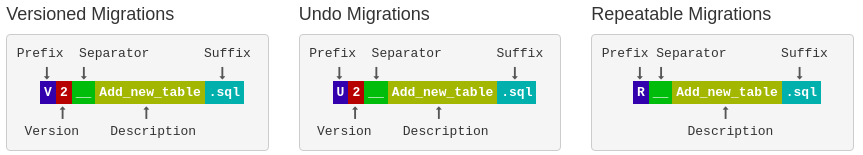
\includegraphics[scale=0.3]{nommage_sql.png}
 % nommage_sql.png: 863x155 px, 72dpi, 30.44x5.47 cm, bb=0 0 863 155
\end{center}

Emplacement des migrations :
\begin{itemize}
 \item classpath: utilisable dans les builds Java avec les plugins Maven et Gradle
 \item filesystem: utilisable avec le cli et les plugins
 \item s3/gcs: à partir de la version 7
\end{itemize}

\begin{center}
 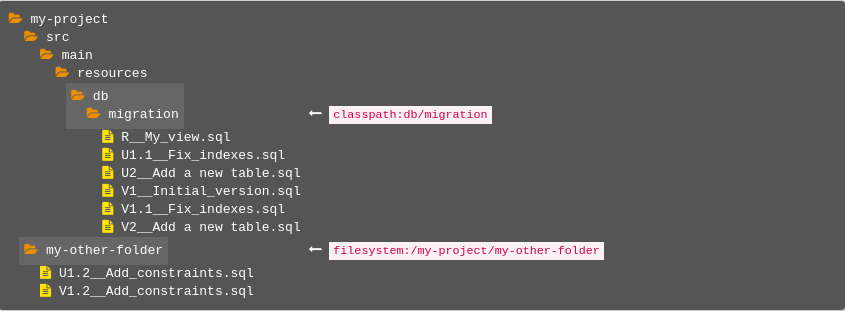
\includegraphics[scale=0.2,keepaspectratio=true]{locations_sql.png}
 % locations_sql.png: 845x312 px, 72dpi, 29.81x11.01 cm, bb=0 0 845 312
\end{center}
\end{frame}

\begin{frame}{Migrations Java}
\setbeamertemplate{itemize/enumerate body begin}{\footnotesize}
Nommage :
\begin{center}
 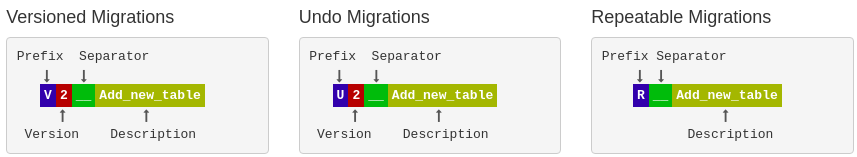
\includegraphics[scale=0.3]{nommage_java.png}
 % nommage_sql.png: 863x155 px, 72dpi, 30.44x5.47 cm, bb=0 0 863 155
\end{center}

Emplacement des migrations :
\begin{itemize}
 \item classpath: utilisable dans les builds Java avec les plugins Maven et Gradle. Il faut compiler les classes avant de lancer la migration.
\end{itemize}

\begin{center}
 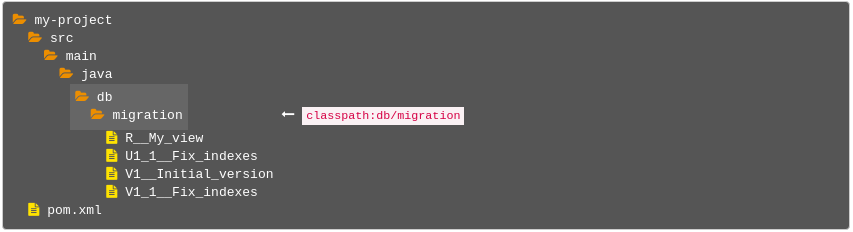
\includegraphics[scale=0.2,keepaspectratio=true]{locations_java.png}
 % locations_sql.png: 845x312 px, 72dpi, 29.81x11.01 cm, bb=0 0 845 312
\end{center}

\end{frame}

\begin{frame}{Table d'historique de schéma}
Pour garder une trace des migrations qui ont déjà été appliquées, Flyway ajoute une table d'historique de schéma. Elle contient les checksums, les temps et l'état d'exécutions des migrations.
\begin{center}
 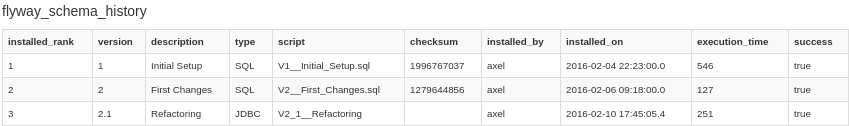
\includegraphics[scale=0.3,keepaspectratio=true]{schema_history_table.png}
 % schema_history_table.png: 849x126 px, 72dpi, 29.95x4.45 cm, bb=0 0 849 126
\end{center}

\textbf{L'aspect transactionnel:} \\
Par défaut, Flyway encapsule l'exécution de chaque migration dans une seule transaction.\\
Il est aussi possible de le configurer pour encapsuler l'exécution complète de toutes les migrations dans une seule transaction.                                                                            

\end{frame}
\subsection*{Fonctionnalités avancées}
\begin{frame}{Fonctionnalités avancées}

Flyway offre plusieurs fonctionnalités avancées: \\
 \begin{itemize}
  \item \textbf{Callbacks}: définir des callbacks en Java/SQL.
  \item \textbf{Error Overrides}: redéfinir le comportement en cas d'erreur (Teams).
  \item \textbf{Dry Runs}: prévisualiser les modifications que Flyway apportera à la BD (Teams).
 \end{itemize}
\end{frame}

\section{Commandes}
\subsection*{Commandes}

\begin{frame}{Migrate/Undo}
\setbeamertemplate{itemize/enumerate body begin}{\footnotesize}
\begin{itemize}
 \item \textbf{Migrate} : migre le schéma vers la dernière version. Flyway créera automatiquement la table d'historique de schéma si elle n'existe pas.
 \item \textbf{Undo} : annule la migration versionnée la plus récemment appliquée (Teams)
\end{itemize}
\vspace{1cm}
Options des commandes migrate/undo:
\begin{itemize}
 \item \textbf{Cherry pick}: spécifiez les migrations à appliquer avec l'option \textit{-cherryPick}. Exemple: \textit{flyway migrate -cherryPick="5,create\_view"}
 \item \textbf{Mark as applied}: avec l'option \textit{skipExecutingMigrations=true}, 
l'exécution du script est ignorée, en mettant à jour la table d'historique de schéma.
\end{itemize}
\end{frame}
\begin{frame}{Info/Validate}
\setbeamertemplate{itemize/enumerate body begin}{\small}
\setbeamertemplate{itemize/enumerate subbody begin}{\footnotesize}
\begin{itemize}
 \item \textbf{Validate} : valide les migrations appliquées par rapport à celles disponibles.
 \item \textbf{Info} : imprime les détails et les informations d'état de toutes les migrations. Les états possibles d'une migration:
    \begin{itemize}
        \item \textbf{success}: la migration est réussie
        \item \textbf{pending}: la migration est détectée et n'est pas appliquée 
        \item \textbf{failed}: lorsque la migration échoue (BD ne supporte pas les transactions) 
        \item \textbf{undone}: la migration versionnée est annulée par la commande undo
        \item \textbf{outdated}: la migration répétable dont le checksum a changé
        \item \textbf{futur}:  la migration versionnée appliquée à une version supérieure à la version la plus élevée connue
    \end{itemize}
\end{itemize}
\end{frame}
\begin{frame}{Clean/Baseline/Repair}
\setbeamertemplate{itemize/enumerate body begin}{\small}
\setbeamertemplate{itemize/enumerate subbody begin}{\footnotesize}
\vspace{1cm}
\begin{itemize}
 \item \textbf{Clean}: supprime tous les objets dans les schémas configurés
 \item \textbf{Baseline}: sert à introduire Flyway dans les bases de données existant en les basant sur une version spécifique.
 \item \textbf{Repair}: répare la table d'historique de schéma en :
    \begin{itemize}
        \item supprimant les entrées de migration ayant échoué
        \item réalignant les checksums, les descriptions et les types des migrations appliquées avec les migrations disponibles
        \item supprimant les migrations répétables supprimées
    \end{itemize}
\end{itemize}
\end{frame}

%%%%%%%%%%%%%%%%%%%%%%%%%%%%%%%%%%%%%%%%%%%%%%%%%%%%%%%%%%%%%%%%%%%%%%%%%%%%%%%%%%%%%%
%% Demo
%%%%%%%%%%%%%%%%%%%%%%%%%%%%%%%%%%%%%%%%%%%%%%%%%%%%%%%%%%%%%%%%%%%%%%%%%%%%%%%%%%%%%%
\section[Démo]{Démonstration}
\subsection*{Scenario 1: exemples de cas d'utilisation de Flyway }
\begin{frame}
Cette démo est réalisé avec une version d'essai Teams:
\begin{enumerate}
 \item Migrate et Undo en SQL 
 \item migration repetables avec chagement de checksum
 \item migration Bash (bulk insert)
 \item migration Java (anonymize)
 \item migration Python 
\end{enumerate}
\end{frame}
\subsection*{Scenario 2: migration Java vs migration à base de Bean Spring}
\begin{frame}
Cette démo est réalisé avec une version d'essai Teams: 
\begin{enumerate}
 \item migration au démarrage de l'application avec l'intégration Spring
 \item migration à base de plain Java: utilisant une connexion JDBC
 \item migration à base de Spring Bean: utilisant Hibernate/ Spring Data
\end{enumerate}
\end{frame}

%%%%%%%%%%%%%%%%%%%%%%%%%%%%%%%%%%%%%%%%%%%%%%%%%%%%%%%%%%%%%%%%%%%%%%%%%%%%%%%%%%%%%%
%% Discussion
%%%%%%%%%%%%%%%%%%%%%%%%%%%%%%%%%%%%%%%%%%%%%%%%%%%%%%%%%%%%%%%%%%%%%%%%%%%%%%%%%%%%%%
\section[Discussion]{Discussion et Q\&A}
\subsection*{Conclusion }
\begin{frame}
\textbf {Pros : \\}
\begin{itemize}
 \item riche en fonctionnalités 
 \item supporte plusieurs langages/platform/BD
 \item facilite les tâches de maintenance pour des cas d'utilisation complexes
\end{itemize}
\textbf {Cons : \\}
\begin{itemize}
 \item l'édition communautaire est limitée 
 \item model de facturation par schéma pour la version Teams
\end{itemize}
\textbf {Alternatives : \\}
\begin{itemize}
 \item Liquibase 
 \item Alembic
 \item Orcas DB
 \item Dbmate
\end{itemize}
\end{frame}

\subsection*{Q\&A et Références}
\begin{frame}
\begin{center}
 
\includegraphics[scale=0.3,keepaspectratio=true]{qa.jpg}
 % qa.jpg: 560x235 px, 100dpi, 14.22x5.97 cm, bb=0 0 403 169
\end{center}

\vspace{1cm}
\begin{itemize}
 \item Documentation : \url{https://flywaydb.org/documentation/} 
 \item Blog : \url{https://flywaydb.org/blog/flyway-7.0.0-beta}
 \item FAQ : \url{https://flywaydb.org/documentation/faq}
\end{itemize}

\end{frame}

\begin{frame}[plain,noframenumbering]
\vspace{2.5cm}
\begin{center} 
\begin{beamercolorbox}[rounded=true,sep=8pt,center]{title}
   	\Huge Merci pour votre attention ! 
		\end{beamercolorbox}%
\end{center} 
\end{frame} 

\end{document}

